% GNUPLOT: LaTeX picture with Postscript
\begingroup
  \makeatletter
  \providecommand\color[2][]{%
    \GenericError{(gnuplot) \space\space\space\@spaces}{%
      Package color not loaded in conjunction with
      terminal option `colourtext'%
    }{See the gnuplot documentation for explanation.%
    }{Either use 'blacktext' in gnuplot or load the package
      color.sty in LaTeX.}%
    \renewcommand\color[2][]{}%
  }%
  \providecommand\includegraphics[2][]{%
    \GenericError{(gnuplot) \space\space\space\@spaces}{%
      Package graphicx or graphics not loaded%
    }{See the gnuplot documentation for explanation.%
    }{The gnuplot epslatex terminal needs graphicx.sty or graphics.sty.}%
    \renewcommand\includegraphics[2][]{}%
  }%
  \providecommand\rotatebox[2]{#2}%
  \@ifundefined{ifGPcolor}{%
    \newif\ifGPcolor
    \GPcolortrue
  }{}%
  \@ifundefined{ifGPblacktext}{%
    \newif\ifGPblacktext
    \GPblacktexttrue
  }{}%
  % define a \g@addto@macro without @ in the name:
  \let\gplgaddtomacro\g@addto@macro
  % define empty templates for all commands taking text:
  \gdef\gplbacktext{}%
  \gdef\gplfronttext{}%
  \makeatother
  \ifGPblacktext
    % no textcolor at all
    \def\colorrgb#1{}%
    \def\colorgray#1{}%
  \else
    % gray or color?
    \ifGPcolor
      \def\colorrgb#1{\color[rgb]{#1}}%
      \def\colorgray#1{\color[gray]{#1}}%
      \expandafter\def\csname LTw\endcsname{\color{white}}%
      \expandafter\def\csname LTb\endcsname{\color{black}}%
      \expandafter\def\csname LTa\endcsname{\color{black}}%
      \expandafter\def\csname LT0\endcsname{\color[rgb]{1,0,0}}%
      \expandafter\def\csname LT1\endcsname{\color[rgb]{0,1,0}}%
      \expandafter\def\csname LT2\endcsname{\color[rgb]{0,0,1}}%
      \expandafter\def\csname LT3\endcsname{\color[rgb]{1,0,1}}%
      \expandafter\def\csname LT4\endcsname{\color[rgb]{0,1,1}}%
      \expandafter\def\csname LT5\endcsname{\color[rgb]{1,1,0}}%
      \expandafter\def\csname LT6\endcsname{\color[rgb]{0,0,0}}%
      \expandafter\def\csname LT7\endcsname{\color[rgb]{1,0.3,0}}%
      \expandafter\def\csname LT8\endcsname{\color[rgb]{0.5,0.5,0.5}}%
    \else
      % gray
      \def\colorrgb#1{\color{black}}%
      \def\colorgray#1{\color[gray]{#1}}%
      \expandafter\def\csname LTw\endcsname{\color{white}}%
      \expandafter\def\csname LTb\endcsname{\color{black}}%
      \expandafter\def\csname LTa\endcsname{\color{black}}%
      \expandafter\def\csname LT0\endcsname{\color{black}}%
      \expandafter\def\csname LT1\endcsname{\color{black}}%
      \expandafter\def\csname LT2\endcsname{\color{black}}%
      \expandafter\def\csname LT3\endcsname{\color{black}}%
      \expandafter\def\csname LT4\endcsname{\color{black}}%
      \expandafter\def\csname LT5\endcsname{\color{black}}%
      \expandafter\def\csname LT6\endcsname{\color{black}}%
      \expandafter\def\csname LT7\endcsname{\color{black}}%
      \expandafter\def\csname LT8\endcsname{\color{black}}%
    \fi
  \fi
  \setlength{\unitlength}{0.0500bp}%
  \begin{picture}(7200.00,5040.00)%
    \gplgaddtomacro\gplbacktext{%
      \csname LTb\endcsname%
      \put(3689,532){\makebox(0,0)[r]{\strut{}-2}}%
      \put(3332,648){\makebox(0,0)[r]{\strut{}-1.5}}%
      \put(2974,764){\makebox(0,0)[r]{\strut{}-1}}%
      \put(2616,880){\makebox(0,0)[r]{\strut{}-0.5}}%
      \put(2257,996){\makebox(0,0)[r]{\strut{} 0}}%
      \put(1899,1113){\makebox(0,0)[r]{\strut{} 0.5}}%
      \put(1541,1229){\makebox(0,0)[r]{\strut{} 1}}%
      \put(1183,1345){\makebox(0,0)[r]{\strut{} 1.5}}%
      \put(825,1461){\makebox(0,0)[r]{\strut{} 2}}%
      \put(6335,1693){\makebox(0,0){\strut{}-2}}%
      \put(6035,1555){\makebox(0,0){\strut{}-1.5}}%
      \put(5734,1416){\makebox(0,0){\strut{}-1}}%
      \put(5434,1278){\makebox(0,0){\strut{}-0.5}}%
      \put(5133,1139){\makebox(0,0){\strut{} 0}}%
      \put(4833,1001){\makebox(0,0){\strut{} 0.5}}%
      \put(4532,862){\makebox(0,0){\strut{} 1}}%
      \put(4232,724){\makebox(0,0){\strut{} 1.5}}%
      \put(3931,585){\makebox(0,0){\strut{} 2}}%
      \put(840,2144){\makebox(0,0)[r]{\strut{}-12}}%
      \put(840,2288){\makebox(0,0)[r]{\strut{}-10}}%
      \put(840,2431){\makebox(0,0)[r]{\strut{}-8}}%
      \put(840,2574){\makebox(0,0)[r]{\strut{}-6}}%
      \put(840,2718){\makebox(0,0)[r]{\strut{}-4}}%
      \put(840,2861){\makebox(0,0)[r]{\strut{}-2}}%
      \put(840,3005){\makebox(0,0)[r]{\strut{} 0}}%
      \put(840,3149){\makebox(0,0)[r]{\strut{} 2}}%
      \put(840,3292){\makebox(0,0)[r]{\strut{} 4}}%
      \put(3600,4621){\makebox(0,0){\strut{}set pm3d hidden3d <linetype>: pm3d's much faster hidden3d variant}}%
    }%
    \gplgaddtomacro\gplfronttext{%
      \csname LTb\endcsname%
      \put(5379,4096){\makebox(0,0)[r]{\strut{}log(x*x*y*y)}}%
      \csname LTb\endcsname%
      \put(6641,2189){\makebox(0,0)[l]{\strut{}-12}}%
      \put(6641,2370){\makebox(0,0)[l]{\strut{}-10}}%
      \put(6641,2551){\makebox(0,0)[l]{\strut{}-8}}%
      \put(6641,2732){\makebox(0,0)[l]{\strut{}-6}}%
      \put(6641,2913){\makebox(0,0)[l]{\strut{}-4}}%
      \put(6641,3094){\makebox(0,0)[l]{\strut{}-2}}%
      \put(6641,3275){\makebox(0,0)[l]{\strut{} 0}}%
      \put(6641,3456){\makebox(0,0)[l]{\strut{} 2}}%
      \put(6641,3638){\makebox(0,0)[l]{\strut{} 4}}%
    }%
    \gplbacktext
    \put(0,0){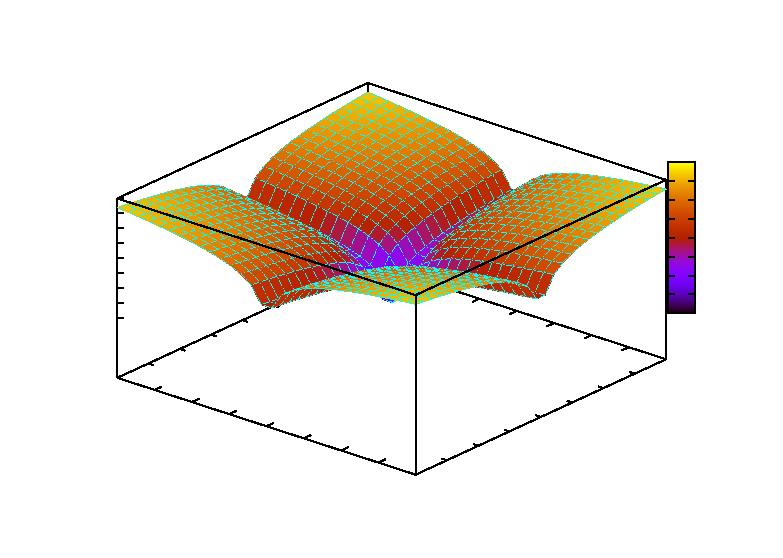
\includegraphics{pm3d17}}%
    \gplfronttext
  \end{picture}%
\endgroup
